The containment of the energy in the supercluster has been verified
with simulations of nuclear and electron recoils performed with
\GEANTfour~\cite{GEANT4} and the gas mixture of the \lemon detector.
For both types of recoils, for the energy range of interest for Dark
Matter search, \ie $E<10$\keV, the median of the
$\abs{E-E_\textrm{true}}/E_\textrm{true}$ is within 5\%. The energy
resolution can be measured in data with \fe source, which provides
monochromatic photons of 5.9\keV, as was described in
Ref.~\cite{bib:fe55}. The distribution of the spot integral, defined as
the sum of the counts of all the pixels belonging to the supercluster,
for a run in presence of \fe source, is shown in
Fig.~\ref{fig:feuncalibpeak}. While to perform the basic- and
super-clustering only pixels passing the zero suppression are
considered, for the energy estimate all the pixels within the cluster
contours are counted, eventually with negative counts, after the
pedestal subtraction. This is done not to induce a bias on the energy
estimate.
%
\begin{figure}[ht]
  \begin{center}
    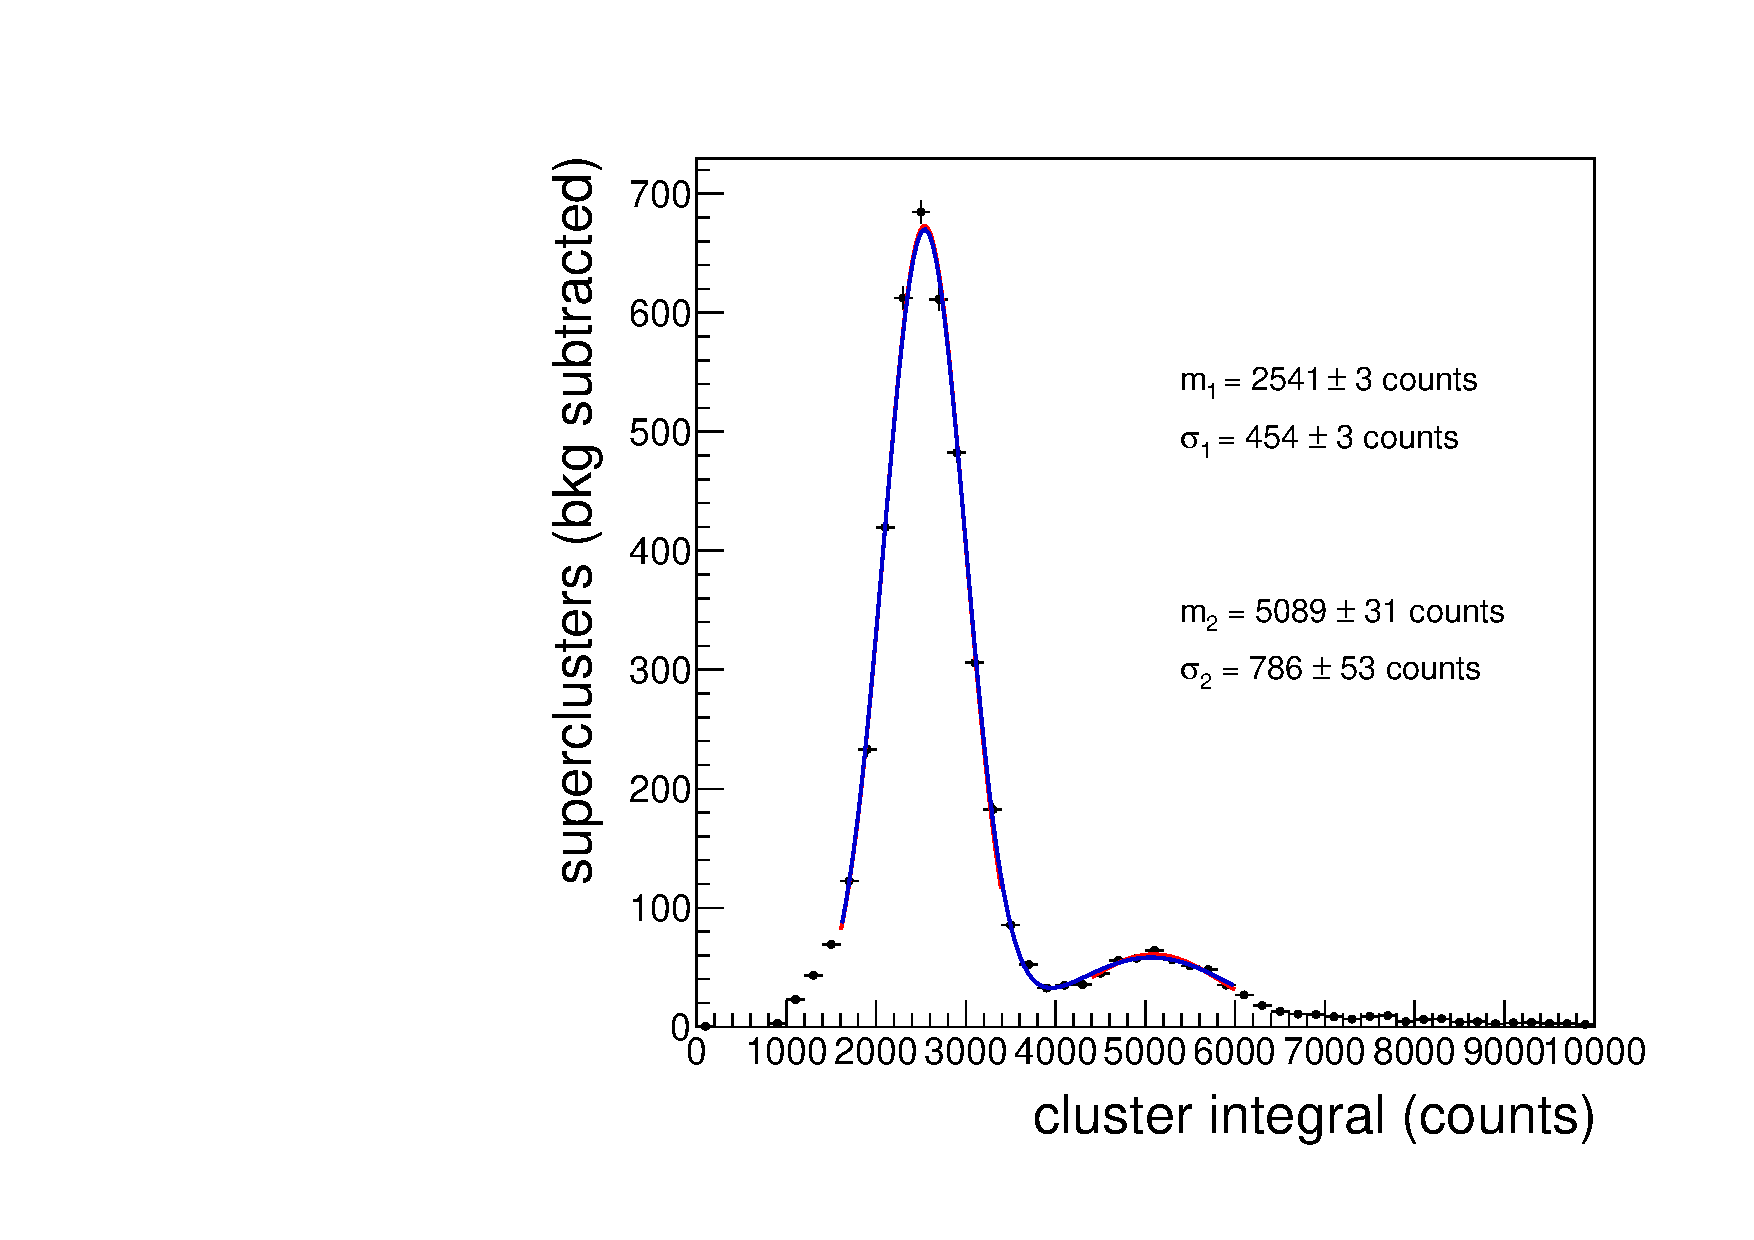
\includegraphics[width=0.49\linewidth]{figures/fe_ucalibintegral_fit}
    \caption{Distribution of the supercluster integral, before the
      absolute energy scale calibration is applied, in events with the
      \fe source. Clearly visible is the large peak of a single spot,
      and, at around twice the energy, a broader peak for the case of
      two neighbor spots merged in a single supercluster.
      \label{fig:feuncalibpeak}}
  \end{center}
\end{figure}
%
The energy resolution for the reconstructed \gac superclusters is
about 18\%, similar to the one that can be obtained with only the
basic clustering step with \idbscan~\cite{iDBSCAN}, and improving the
one with the simple NNC algorithm previously used for the CYGNO
experiment~\cite{bib:fe55}.



